\chapter{Fejlesztői dokumentáció} % Developer guide
\label{ch:impl}

Ez a fejezet fejlesztőknek nyújt segítséget a ScrumHelper feltérképezésében. Az alfejezetek kifejtik az alkalmazás felépítését, részletesen leírják a különböző rétegeinek (Adatbázis-Szerver-Nézet) osztályait és függvényeit. A vizuális segítséghez különböző diagrammokat is tartalmaz (osztály-, csomag-, felhasználói esetek diagram). A fejezet végén egy tesztforgatókönyv ad részletes leírást a teszt esetek és azok elvárt eredményeiről.

\section{Konfiguráció, fejlesztői környezet}
\label{config}

A futtatáshoz szükséges előkövetelmények a felhasználói dokumentáció \ref{install}. alfejezetében olvashatók. A dolgozat keretein belül csak a lokális szerveren való konfigurálás és futtatás lesz részletezve. A különböző szervergépeken való futtatáshoz részletesebb információt a hivatalos Django dokumentációban lehet találni. Utóbbi eset külön konfigurációt igényel a wsgi.py, illetve asgi.py file-ok és környezeti változók megfelelő beállításának segítségével \footnote{wsgi szerver: \url{https://docs.djangoproject.com/en/3.0/howto/deployment/wsgi/}} \footnote{asgi szerver: \url{https://docs.djangoproject.com/en/3.0/howto/deployment/asgi/}}.  

Ahhoz, hogy lokálisan futtatni tudjuk a szervert, először is a ScrumHelper/ScrumHelper/setting.py file-ban kell beállítanunk a DATABSES változót. A pontos beállításai eltérőek a különböző adatbázisok esetében, ehhez részletes segítséget nyújt a hivatalos Django dokumentáció. Alább  egy PostgreSQL adatbázis konfigurációja látható:

\lstset{caption={Konfiguráció PostgreSQL adatbázis használatához}, label=src:settingsconf}
\begin{lstlisting}[language={python}]

DATABASES = {
    'default': {
        'ENGINE': 'django.db.backends.postgresql',
        'NAME': 'database name',
        'USER': 'database user',
        'PASSWORD': 'password',
        'HOST': '127.0.0.1',
        'PORT': '5432',
    }
}

\end{lstlisting}

Ha ez megfelelően van beállítva, akkor a ScrumHelper fő mappába navigálva kell lefuttatni a" python manage.py migrate" parancsot minden első futtatásnál a szükséges adatbázis struktúra kialakításához(illetve ha fejlesztés során olyasmi változik, amely érinti az adatbázis struktúrát, akkor a makemigrations-t is le kell a migrate parancs előtt futtatni). Ezután a "python manage.py runserver" elindítja a lokális szervert a localhost:8000-es portján. Superuser-t, azaz minden jogosultsággal rendelkező felhasználót a szerver futtatása nélkül lehet generálni: "python manage.py createsuperuser" paranccsal, megadva a felhasználónevet és jelszavat utána.

A TIMEZONE változóban adható meg az időzóna. Az egyes projektekhez feltöltött fájlokat a MEDIA\_ROOT konfigurációs változóbeli elérési úton elhelyezkedő mappába menti (ez alapból a ScrumHelper/media könyvtárra mutat). Ugyanezen az elven kezeli a statikus fájlokat is a keretrendszer, ennek a környezeti változója a STATIC\_ROOT.

Fontos, hogy mielőtt az alkalmazás valós, produkciós használatba kerülne szükséges a DEBUG változót False-ra, azaz hamisra állítani (biztonásgi okokból). Utóbbi azért is fontos, mert így a szerver nem küld debug információkat a kliensre.

A Django nem rendelkezik saját fejlesztői környezettel, így bármely python fejlesztésre alkalmas IDE használható. Például a Visual Studio Code rendelkezik minden bővítménnyel, amely szükséges lehet egy Django alkalmazás futtatásához, valamint egyéb "kényelmet" segítő funkciókkal is (szintaxis ellenőrzés/kiemelés Pythonhoz/HTML-hez/CSS-hez/JavaScript-hez és a Django template-khez). A szükséges szoftverek (\ref{install}) megléte mellett akár egy egyszerű szövegszerkeztő alkalmazás is elegendő (de célszerűbb valamilyen integrált fejlesztői környezetet használni).

\section{Funkcionális terv}

Az \ref{fig:usecase}. ábrán egy felhasználói eset diagram mutatja be az alkalmazás funkcióit:

\begin{figure}[H]
	\centering
	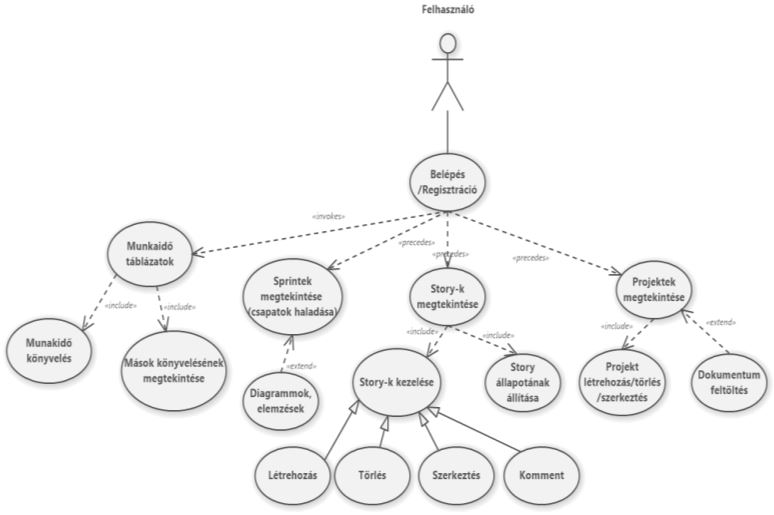
\includegraphics[scale=0.95]{usecase}
	\caption{Felhasználói eset diagram}
	\label{fig:usecase}
\end{figure}

\section{Struktúrális felépítés}

A ScrumHelper egy MVC (Model-View-Controller) alkalmazás, bár a hivatalos Django dokumentációban az MTV (Model-Template-View) kifejezést használják, mivel ezt gondolják pontosabb leírásának. Tekintve, hogy Djangoban írodott az alkalamzás, ezért ebben a dokumentációban is utóbbi analógia az irányadó. Ez azt jelenti, hogy három rétegből tevődik össze: egy Model rétegből, amely az adatbázist hivatott reprezentálni, egy View rétegből, amely az adatot reprezentálja (ez alatt azt értjük, amit az adatbázisből kigyűjtött, nem feltétlenül a felhasználó számára megjelenített adatot), valamint a különböző template-ek renderelését is végzi, továbbá egy Template rétegből, mely definiálja, hogyan legyen az adat megjelenítve a felhasználó számára.

\begin{figure}[H]
	\centering
	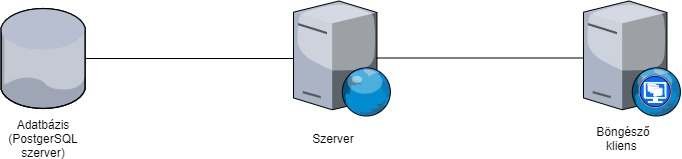
\includegraphics[width=1\textwidth,height=125px]{architecture}
	\caption{Az alkalamzás rétegei: egy adatbázis, egy szerver, ami kinyeri belőle az adatot és továbbítja a nézetnek, valamint a nézet amit a böngészőben láthatunk.}
	\label{fig:architecture}
\end{figure}

A django alkalmazások úgynevezett applikációkból állnak, amelyek a moduláris felépítést segítik elő. Ezek gyakorlatilag a python nyelvből ismert csomagokkal -package-ekkel- egyeznek meg. A \ref{fig:packages}. ábra szemléletesebben bemutatja ezen applikációkat (modulokat) és azok kapcsolatait:

\begin{figure}[H]
	\centering
	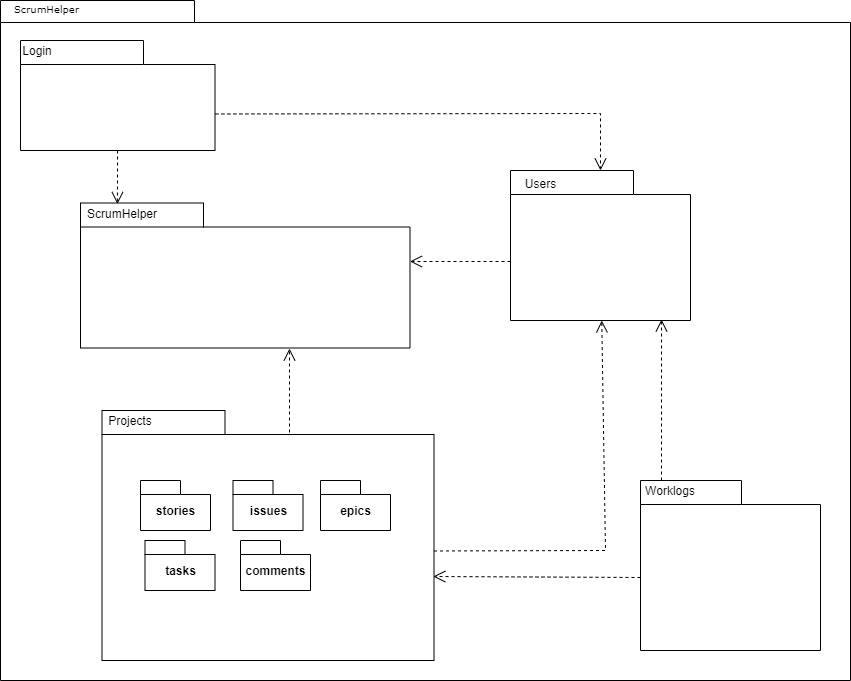
\includegraphics[width=1\textwidth,height=300px]{scrumhelperPackage}
	\caption{Csomagdiagramm}
	\label{fig:packages}
\end{figure}

\pagebreak

\begin{itemize}
 	\item Ahogy az ábrán is látható, a fő csomag a ScrumHelper. Ez fogja össze működésben az alkalamzást.
	\item A legnagyobb applikáció a "Projects", ugyanis ez tartalmazza egyben a "Stories", "Tasks", "Issues", "Comments", "Epics" applikációkat is.
	\item A felhasználók kezelésével foglalkozó csomag a "Users" és részben a "Login". Utóbbi a ki- és bejelentkeztetésre, valamint a felhasználók regisztrálására és szerkeztésére szolgál.
	\item Egy kisebb alkalmazás, a "Worklogs" adja a modell szintű reprezentációját a munkaidő naplónak.
\end{itemize}

Ezek implementáció, részletei a későbbi alfejezetekben olvashatóak. 

\section{Adatbázis réteg}
\label{dbmodels}

A django keretrendszernek köszönhetően érdemben nem számít, hogy milyen adatbázissal dolgozunk (legalábbis az adatbázis kezelés szempontjából). A ScrumHelper fejlesztése során a nyílt-forráskódú PostgreSQL-re esett a választás, de a python modellek és az adatbázis lekérdezések függetlenek attól, hogy milyen adatbázist használunk. Ha csak egy kis, egyszerű alkalmazás megvalósítása a cél akkor érdemesebb például SQLite adatbázist használni, tekintve, hogy az csak egy lokális fájlban tárolja az adatokat, könnyebb menedzselni. A PostgreSQL (a MySQL, Oracle, MariaDB mellett) jobb döntésnek bizonyul nagyobb méretű alkalmazások esetén. 

Az egyes adatbázis táblákat (entitásokat) egy-egy modell reprezentál a forráskódban. Ezek a django.db.models.Model osztályból vannak származtatva. Az egyes modellek attribútumai egy-egy oszlopot reprezentálnak a táblában. A django dokumentációban\footnote{django modell típusosztályok: \url{https://docs.djangoproject.com/en/3.0/ref/models/fields/}} részletes leírás található arról, mely mezőtípusokhoz milyen paramétereket lehet megadni ahhoz, hogy minél jobban testreszabhassuk a mező tulajdonságait. Van lehetőség modell szintű metódusokat is definiálni ugyanúgy, mint a python osztályoknál (hiszen ezek is python osztályok), de ezek nem lesznek jelen az adatbázisban. A modell szinten jellemzően csak egyszerűbb metódusokat szokás definiálni, mint például az \textit{\_\_str\_\_()} felüldefiniálása a felsőbb rétegek segítségéül, vagy az \textit{\_\_init\_\_} inicializációs függényt. Érdemes azonban kerülni az ilyen megoldásokat, hogy minél jobban elszeparálhatóak legyenek az egyes rétegek.  A következő alfejezetekben részletes információk találhatóak az egyes modellekről.

\subsection{Felhasználó kezelés: Users, Login modellek}

\begin{figure}[H]
	\centering
	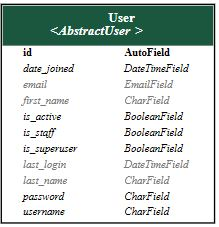
\includegraphics[scale=1.5]{userModel}
	\caption{User modell diagrammja}
	\label{fig:usermodel}
\end{figure}

A \textbf{django.contrib.auth.models.User} modell reprezentál egy-egy felhasználót. Ez magában a keretrendszerben megtalálható. Elég sokoldalú, de van lehetőség kiegészíteni, esetlegesen helyettesíteni saját megvalósítással is. Kiegészítésre példa a \textbf{Profile} modell osztály a users applikációban. Egy \textbf{OneToOneField} segítségével és szignálokkal (\textit{create\_user\_profile} és \textit{save\_user\_profile}) tudjuk az eredeti \textbf{Users} osztályhoz kötni. A szignálok azért szükségesek, mert így tud a modell reagálni az eredeti modell esetleges változásaira (létrehozás, módosítás, törlés). A mezők:

\begin{itemize}
	\item \textit{id}: mezőazonosító (alapvetően generált)
	\item \textit{date\_joined}: beregisztrálás dátuma
	\item \textit{email}: email cím
	\item \textit{first\_name}: keresztnév
	\item \textit{is\_active}: nem zárolt-e a felhasználó (azaz inaktív)
	\item \textit{is\_staff}: adminisztrátor-e
	\item \textit{is\_superuser}: Minden jogosultsággal rendelkező felhasználó-e
	\item \textit{last\_login}: utolsó bejelentkezés dátuma
	\item \textit{last\_name}: vezeték név
	\item \textit{password}: jelszó (hashelve, azaz kódolva)
	\item \textit{username}: felhasználónév
\end{itemize}

A \textbf{Login} modul nem rendelkezik külön adatbázis reprezentációval, mivel a \textbf{User} modelljét használja föl.

\subsection{Project modell}

\begin{figure}[H]
	\centering
	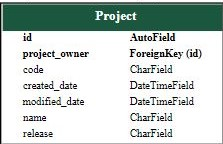
\includegraphics[scale=1.5]{projectModel}
	\caption{Project modell diagrammja}
	\label{fig:projectmodel}
\end{figure}

A \textbf{Projects} applikáció saját adatbázis modellje a \textbf{Project}:

\begin{itemize}
	\item \textit{id}: mezőazonosító (alapvetően generált)
	\item \textit{project\_owner}: a projektet létrehozó felhasználó (idegen kulcs a \textbf{Users} táblára)
	\item \textit{code}: a projekt 6 karakter hosszú kódja (egyedi kell legyen)
	\item \textit{created\_date}: a létrehozás dátuma
	\item \textit{modified\_date}: az utolsó módosítás dátuma
	\item \textit{name}: a projekt neve (maximum 50 karakter hosszú)
	\item \textit{release}: a Release neve (maximum 10 karakter hosszú)
\end{itemize}

Rendelekezik egy \textit{documents} attribútummal is, mely egy \textbf{ManyToManyField} típusú mező, azaz több idegen kulcs kapcsolatot fog egybe (erre a célra a django automatikusan létrehoz egy táblát, amelyben benne lesznek ezek az összekapcsolások) a \textbf{Documents} modell táblájának \textit{id} mezőjével. Ennek seígtségével kapcsolódik egy adott projekthez több dokumentum is.

\begin{figure}[H]
	\centering
	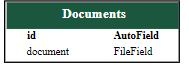
\includegraphics[scale=1.5]{documentModel}
	\caption{Documents modell diagrammja}
	\label{fig:docmodel}
\end{figure}

A \textbf{Documents} modell rendelkezik egy \textit{document} attribútummal, mely \textbf{FileField} típusú. Ez a típusosztály reprezentálja Djangoban a fájl mezőket az adatbázisban. A fájl relatív elérési útját menti le az adatbázisba. Jelen alkalmazásban a \textit{documents/} mappát használja, de ez is konfigurálható a \textit{projects.models.project\_directory\_path(instance, filename)} függvény segítségével. A visszatérési értékben (amely egy string) lehet megadni az elérési utat.

\subsection{Epic modell}

\begin{figure}[H]
	\centering
	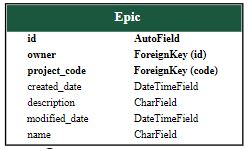
\includegraphics[scale=1.5]{epicModel}
	\caption{Epic modell diagrammja}
	\label{fig:epicmodel}
\end{figure}

Az \textbf{Epic} a \textit{project\_code} mezővel kapcsolódik a \textbf{Project} tábla \textit{code} mezőjéhez. Egy projekthez több több epic is tartozhat, de egy epic csak egy projekthez kapcsolódhat. Ha a projekt törlődik, vagy a létrehozó felhasználó, akkor az összes epic is amelyek hozzá tartoznak. A modell mezői:

\begin{itemize}
	\item \textit{id}: mezőazonosító (alapvetően generált)
	\item \textit{owner}: az epic-et létrehozó felhasználó (idegen kulcs a \textbf{Profile} táblára)
	\item \textit{project\_code}: a projekt 6 karakter hosszú kódja (idegen kulcs, a \textbf{Project} tábla \textit{code} mezőjére mutat)
	\item \textit{created\_date}: a létrehozás dátuma
	\item \textit{modified\_date}: az utolsó módosítás dátuma
	\item \textit{name}: az epic neve (maximum 50 karakter hosszú)
	\item \textit{description}: egy leírás az epic-ről (maximum 250 karakter hosszú)
\end{itemize}

\subsection{Story modell}

\begin{figure}[H]
	\centering
	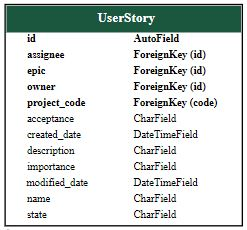
\includegraphics[scale=1.5]{storyModel}
	\caption{Story modell diagrammja}
	\label{fig:storymodel}
\end{figure}

A \textbf{UserStory} több táblához is rendelkezik idegen kulccsal: kapcsolódik egyrészt a projekthez, amely alatt létrehozták, kapcsolódik továbbá a felhasználóhoz, aki létrehozta, illetve akihez rendelve van (opcionális), valamint kapcsolódik egy epic-hez (ez is opcionális). Egy story csak addig létezik, amíg a projekt is, amely alatt létehozták, avagy ki nem törlik. Ha epic-hez van rendelve és töröljük, akkor csak kinullázódik azon mezője. Abban az esetben, ha a felhasználót töröljük, aki létrehozta a story-t, akkor is törlődik. A modell mezői:

\begin{itemize}
	\item \textit{id}: mezőazonosító (alapvetően generált)
	\item \textit{assignee}: idegen kulcs a hozzárendelt felhasználóra (lehet üres, \textbf{User} tábla)
	\item \textit{epic}: idegen kulcs az \textbf{Epic} táblára (lehet üres)
	\item \textit{owner}: az story-t létrehozó felhasználó (idegen kulcs a \textbf{Profile} táblára)
	\item \textit{project\_code}: a projekt 6 karakter hosszú kódja (idegen kulcs, a \textbf{Project} tábla \textit{code} mezőjére mutat)
	\item \textit{acceptance}: feladattal kapcsolatos elvárások leírása, amelyeknek teljesülnie kell (például teszt során, maximum 50 karakter)
	\item \textit{created\_date}: a létrehozás dátuma
	\item \textit{modified\_date}: az utolsó módosítás dátuma
	\item \textit{name}: a story neve (maximum 50 karakter hosszú)
	\item \textit{description}: egy leírás a story-ról (maximum 250 karakter hosszú)
	\item \textit{importance}: fontosság (Low, Medium, High)
	\item \textit{state}: aktuális állapot (OPEN, IN PROGRESS, TESTING, DONE, CLOSED)
\end{itemize}

Rendelkezik egy \textit{comment} mezővel is, amely több kommentet is össze kapcsol egy \textbf{UserStory}-val (\textbf{ManyToMany} reláció, külön kapcsolati táblával). Ugyanilyen kapcsolatban áll a \textbf{Worklog} táblával is a \textit{work\_log} mezőn keresztül.

\subsection{Task modell}

\begin{figure}[H]
	\centering
	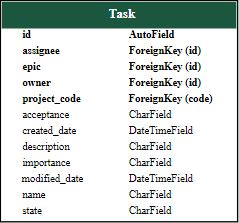
\includegraphics[scale=1.5]{taskModel}
	\caption{Task modell diagrammja}
	\label{fig:taskmodel}
\end{figure}

A \textbf{Task} modell felépítése szinte megegyezik a \textbf{UserStory}-éval. Ugyanúgy egy projekthez, esetlegesen egy epic-hez és a létrehozó felhasználóhoz kapcsolódik (és opcionálisan akihez hozzá van rendelve). Az eltérés a státuszaiban van: csak OPEN (nyitott), DONE(kész) és CLOSED(lezárt) lehet. A mezői:

\begin{itemize}
	\item \textit{id}: mezőazonosító (alapvetően generált)
	\item \textit{assignee}: idegen kulcs a hozzárendelt felhasználóra (lehet üres, \textbf{User} tábla)
	\item \textit{epic}: idegen kulcs az \textbf{Epic} táblára (lehet üres)
	\item \textit{owner}: az task-ot létrehozó felhasználó (idegen kulcs a \textbf{Profile} táblára)
	\item \textit{project\_code}: a projekt 6 karakter hosszú kódja (idegen kulcs, a \textbf{Project} tábla \textit{code} mezőjére mutat)
	\item \textit{acceptance}: feladattal kapcsolatos elvárások leírása, amelyeknek teljesülnie kell (például teszt során, maximum 50 karakter)
	\item \textit{created\_date}: a létrehozás dátuma
	\item \textit{modified\_date}: az utolsó módosítás dátuma
	\item \textit{name}: a task neve (maximum 50 karakter hosszú)
	\item \textit{description}: egy leírás a task-ról (maximum 250 karakter hosszú)
	\item \textit{importance}: fontosság (Low, Medium, High)
	\item \textit{state}: aktuális állapot (OPEN, DONE, CLOSED)
\end{itemize}

Rendelkezik egy \textit{comment} mezővel is, amely több kommentet is össze kapcsol egy \textbf{Task}-kal (\textbf{ManyToMany} reláció, külön kapcsolati táblával). Ugyanilyen kapcsolatban áll a \textbf{Worklog} táblával is a \textit{work\_log} mezőn keresztül.

\subsection{Issue modell}

\begin{figure}[H]
	\centering
	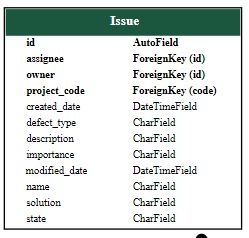
\includegraphics[scale=1.5]{issueModel}
	\caption{Issue modell diagrammja}
	\label{fig:issuemodel}
\end{figure}

Az \textbf{Issue} modellje már több mezőben is eltér a \textbf{Task} és \textbf{UserStory}-tól. A plusz mezők a korábbiakhoz képest, a \textit{defect\_type} és \textit{solution}. Előbbi a hiba típusát hívatott reprezentálni, utóbbi pedig egy rövid leírás a megoldásról. Ez is kapcsolódik egy projekthez és a létrehozójához, valamint ahhoz akihez hozzárendelik (opcionális).

\begin{itemize}
	\item \textit{id}: mezőazonosító (alapvetően generált)
	\item \textit{assignee}: idegen kulcs a hozzárendelt felhasználóra (lehet üres, \textbf{User} tábla)
	\item \textit{owner}: az issue-ot létrehozó felhasználó (idegen kulcs a \textbf{Profile} táblára)
	\item \textit{project\_code}: a projekt 6 karakter hosszú kódja (idegen kulcs, a \textbf{Project} tábla \textit{code} mezőjére mutat)
	\item \textit{created\_date}: a létrehozás dátuma
	\item \textit{defect\_type}: a hiba típusa (BUG, SYSTEM DEFECT - rendszer szintű, SPECIFICATION ISSUE - tervezési hiba, DEVELOPMENT ISSUE - fejlesztési hiba)
	\item \textit{modified\_date}: az utolsó módosítás dátuma
	\item \textit{name}: az epic neve (maximum 50 karakter hosszú)
	\item \textit{description}: egy leírás az issue-ról (maximum 250 karakter hosszú)
	\item \textit{importance}: fontosság (Low, Medium, High)
	\item \textit{soultion}: a megoldás rövid leírása (maximum 150 karakter)
	\item \textit{state}: aktuális állapot (OPEN, IN PROGRESS, TESTING, DONE, CLOSED)
\end{itemize}

Rendelkezik egy \textit{comment} mezővel is, amely több kommentet is össze kapcsol egy \textbf{Issue}-val (\textbf{ManyToMany} reláció, külön kapcsolati táblával). Ugyanilyen kapcsolatban áll a \textbf{Worklog} táblával is a \textit{work\_log} mezőn keresztül.

\subsection{Comment modell}

A \textbf{Projects} applikáción belül található a \textbf{Comments} modul is. Egy-egy \textbf{UserStory, Task, Issue} rendelkezhet kommentekkel különböző felhasználóktól. Ezekhez az egyes modellekben van idegen kulcsos mező, amely mutat egy-egy kommentre (\textbf{Many-To-Many} kapcsolat). 

\begin{figure}[H]
	\centering
	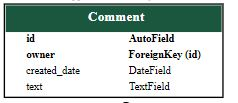
\includegraphics[scale=1.5]{commentModel}
	\caption{Comment modell diagrammja}
	\label{fig:commentModel}
\end{figure}

Mezői:

\begin{itemize}
	\item \textit{id}: mezőazonosító (alapvetően generált)
	\item \textit{owner}: a kommentelő felhasználó (idegen kulcs a \textbf{User} táblára)
	\item \textit{created\_date}: a létrehozás dátuma
	\item \textit{text}: a komment szövege (maximum 250 karakter hosszú)
\end{itemize}

\subsection{Worklog modell}

\begin{figure}[H]
	\centering
	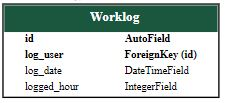
\includegraphics[scale=1.5]{worklogModel}
	\caption{Worklog modell diagrammja}
	\label{fig:worklogmodel}
\end{figure}

A munkaidő napló adatbázis reprezentációjául a \textbf{Worklog} modell szolgál. Munkaidő napló bejegyzést \textbf{UserStory-hoz, Task-hoz és Issue-hoz} tudunk létrehozni. Ezekhez az egyes modellek saját \textit{work\_log} mezőjével kapcsolódik. A mezői:

\begin{itemize}
	\item \textit{id}: mezőazonosító (alapvetően generált)
	\item \textit{log\_user}: a létrehozó felhasználója (idegen kulcs a \textbf{User} táblára)
	\item \textit{log\_date}: a létrehozás dátuma
	\item \textit{logged\_hour}: az órák száma ([0..8] intervallumba kell essen)
\end{itemize}

\section{Szerver réteg}

A szerver réteg jelen alkalmazásban a szolgáltatások (services) és nézetek (views) adják. Egy-egy applikáció a következő modulokból (gyakorlatilag fájlokból épül fel):

\begin{itemize}
	\item \textit{admin.py}: A Django biztosít egy admin felületet az alkalmazás adatbázis szintű kezelésére. Egy adott modell akkor szerkezthető az admin oldalon, ha beregisztráljuk ebben a fájlban.
	\item \textit{apps.py}: Az egyes applikációk nevét tudjuk itt megadni, amivel tudunk rá hivatkozni a többi alkalmazásból (például: "projects.stories"), valamint egyéb alapkonfigurációkat az applikációról.
	\item \textit{migrations}: Ez egy almappa, amiben alap és későbbi (fájl nevében időponttal jelölt) adatbázis migrációk találhatók. Ezek a modellek változásaikor az adatbázis reprezentációjukon módosítanak annak megfelelően.
	\item \textit{templates}: A template-eket, azaz a HTML fájlokat tartalamzza, amik a böngészőben megjelenítendő Nézet rétehet adják. Lehetőség van a fő mappában (jelen esetben \textit{ScrumHelper}) létrehozni egyetlen tempaltes mappát és abban alkalamzásonként almappát, amelybe helyezzük a fájlokat,   de az újrafelhasználhatóság érdekében jobb megoldás minden ilyen fájlt és almappát az applikáció saját mappájában elhelyezni.
	\item \textit{constants.py}: nem kötelező fájl. Applikáció szintű konstansok tárolására használható.
	\item \textit{forms.py}: Szintén nem kötelező fájl. Ha használunk form-okat (például regisztrációra), akkor érdemes ebbe a fájlba elhelyezni ezeket.
	\item \textit{services.py}: A szolgáltatások helye. Ez sem kötelező, de ha az alkalamzáshoz például egy API-t (Application Programming Interface) akarunk fejelszteni, akkor helyesebb analógia a view-k helyett service-eket használni.
	\item \textit{tests.py}: Az egyes applikációk egységteszt modulja.
	\item \textit{views.py}: A view-k (nézetek) modulja. Ezek jelentik a közvetlen kapcsolatot az adatbázis/szolgáltatás réteg és a template-ek (a megjelenítés) között. A view függvények mindig kapnak egy \textit{request} paramétert bemenetként, amiben a hívás adatai vannak (például form esetén az adatok, vagy fájlok, stb.).
	\item \textit{urls.py}: Az applikációk szolgáltatásainak és view-inak az elérési útját tartalmazza (azaz a végpontokat, URL címeket).
\end{itemize}

A következő alfejezetekben az egyes applikációk szerver rétegébe tartozó részei lesznek részletezve (szolgáltatások, nézetek, végpontok, formulák).

\subsection{Login applikáció}

A \textbf{Login} applikáció a bejelentkeztetésért felelős. Alapvetően a keretrendszerben implementált bejelentkeztetést használja, illetve azt bővíti ki.

\begin{itemize}
	\item \textbf{Forms:}

	\begin{description}
		\item[SignUpForm:] A regisztrációs formula. \textbf{UserCreationForm}-ból van származtatva, amely a \textit{django.contrib.auth.forms} modulban van implementálva. A formulának hét mezője van: \textit{username, first\_name, last\_name, email, password1, password2, group}. Vannak megkötések az egyes mezőkre. A \textit{first\_name} csak 30 karakter hosszú lehet, nem kötelező megadni. Ugyanezek igazak a \textit{last\_name} mezőre is. Az \textit{email} mező egy maximum 254 karakter hosszú, email formátumú bemenetet fogad csak el. A \textit{password1} és \textit{password2} mezők jelszó mezők, amiknek egyezniük kell a formula véglegesítésekor. A \textit{group} egy olyan mezőtípus (\textbf{ChoiceField}, amely közvetlenül az adatbázisból kérdezi le a választási lehetőségeket (az \textit{auth\_groups} táblából).
		\item[ChangePassword:] A jelszóváltoztatáshoz használt formula. Ugyanazokkal a mezőkkel rendelkezik, mint a regisztrációs formula.
	\end{description}

	\item \textbf{Nézetek (views):}

	\begin{description}
		\item[CustomLoginView:] Erre azért van szükség, mert itt tudjuk megadni a \textit{redirect\_filed\_name} attribútummal, hogy hova navigáljon bejelenkezés után (jelen esetben: users/index.html).
		\item[index:] Az index oldal, azaz a "login/index.html" tartalmát jeleníti meg. 
\textbf{Végpontja:} "/" avagy "/login".
		\item[logout:] Meghívja a  \textit{django.contrib.auth.login} függvényt és visszanavigál a \textit{login} oldalra. 
\textbf{Végpontja:} "/logout/".
		\item[signup:] A regisztrációs formula segítségével biztosítja a felahsználó létrehozását. A "POST" HTTP üzenetet kap bemenetként, akkor ellenőrzi, hogy helyes-e a formula, majd lementi a felahsználót és hozzárendeli a megfelelő csoporthoz. Ezután visszajuttat az aktuálisan bejelentkezett felhasználó index oldalára. "GET" üzenet esetén csak egy üres forumlát biztosít kitöltésre a \textit{registration/signup.html} számára. 
\textbf{Végpontja:} "registration/signup/".
		\item[edit\_user:] Az egyes felhasználók szerkeztésére szolgál. Ugyanazt a formulát ahsznála, mint a regisztráció, csak itt "GET" üzenet esetén is a az ismert adatokkal kitöltve adja át a tempalte-nek. 
\textbf{Végpontja:} "edit\_user/<int:user\_id>/", azaz a bemenő paramétere egy felhasználói azonosító.
		\item[change\_pw:] A jelszóváltoztatást valósítja meg. Ehhez szintén egy user\_id-t vár bementként és a regisztrációs formulát használja. Azért van szükség mégis külön kezelni, mert nem midne felhasználónak van jogosultsága elérni a szerkeztést. 
\textbf{Végpontja:} "change\_pw/<int:user\_id>".
	\end{description}
\end{itemize}

\subsection{Projects applikáció}

A \textbf{Projects} applikáció a projektek megvalósítása. Ennek almappái a \textbf{Stories, Issues, Comments, Tasks, Epics} applikációk, de ezek külön fejezetkben leszek részletezve. A \textbf{Comments} applikáció lényegében csak a kommentek adatbázis reprezentációjára szolgál, saját szolgáltatásokkal és nézettel nem rendelkezik, így ez nem lesz részletezve ebben a fejezetben.

\begin{itemize}
	\item \textbf{Forms:}
	\begin{description}
		\item[CreateProjectForm:] A projekt létrehozásához használatos form. Mezői: \textit{name, code, release}, azaz a projekt neve, a projekt 6 karakter hosszú kódja és a release kódja.
		\item[CreateStoryForm:] A \textbf{Story} létrehozás form-ja. Mezői: \textit{name, project\_code, assignee, description, importance, epic}. A \textit{project\_code, assignee, epic} mezők \textbf{ModelChoiceField} típusúak, tehát egy megadott adathalmazból kínálnak fel opciókat. Az \textit{epic} és \textit{assignee} mezők kiválasztása nem kötelező.
		\item[CommentForm:] A kommentek létrehozásához használt form. Csak \textit{text} mezője van a komment szövegének lementéséhez.
		\item[CreateEpicForm:] Az \textbf{Epic} létrehozó formulája. Mezői: \textit{name, project\_code, description}, azaz a neve, a projekt kódja, amelyhez tartozik és egy leírás.
		\item[CreateWorklogform:] A \textbf{Worklog}, azaz munkanapló bejegyzés létrehozásához használt form. Mezők: \textit{log\_date, logged\_hour}. A feladattal végzett munkaidő és maga a munkanap.
		\item[CreateTaskForm:]  A \textbf{Task} létrehozás form-ja. Mezői: \textit{name, project\_code, assignee, description, importance, epic}. A \textit{project\_code, assignee, epic} mezők \textbf{ModelChoiceField} típusúak, tehát egy megadott adathalmazból kínál fel opciókat. Az \textit{epic} és \textit{assignee} mezők kiválasztása nem kötelező.
		\item[CreateIssueForm:] Az \textbf{Issue} létrehozás form-ja. Mezői: \textit{name, project\_code, assignee, description, importance, epic, defect\_type,solution}. A \textit{project\_code, assignee, epic} mezők \textbf{ModelChoiceField} típusúak, tehát egy megadott adathalmazból kínál fel opciókat. Az \textit{epic} és \textit{assignee} mezők kiválasztása nem kötelező. A \textit{defect\_type} mező is egy \textbf{ChoiceField}, tehát adott lehetőségekből lehet választani: BUG, SYSTEM DEFECT, DEVELOPMENT, SPECIFICATION ISSUE. Utóbbi értékek egy konstansban találhatóak a \textit{contants.py} modulban, az \textit{ISSUE\_CHOICES} változóban.
	\end{description}
	\item \textbf{Szolgáltatások (services):}
	\begin{description}
		\item[get\_issues\_for\_project:] Bemeneti paramétere: \textit{project\_id}. A megkapott projekt azonosítóhoz lekérdezi magát a projektet, a hozzátartozó story-kat, task-okat, issue-kat, epic-eket és feltöltött dokumentumokat. Ezeket egy \textit{context} nevű, dictionary típusú változóba gyűjti, ami a visszatérési értéke a függvénynek.
		\item[delete\_project:] Bemeneti paraméter: \textit{project\_id}. A megkapott projekt azonosító alapján megkeresi az adatbázisban a projektet és kitörli.
	\end{description}
	\item \textbf{Nézetek (views):}
	\begin{description}
		\item[index:] Lekérdezi az adatbázisban található összes projektet. A \textit{django.core.paginator} modul beli \textbf{Paginator} segítségével oldalakra osztja az eredményeket (jelen beállítás szerint ötösével). Ennek megoldása a \ref{src:paginator}. kódrészletben látható. Az így rendezett projekt listát hozzárendeli a "projects/index.html"-hez. \textbf{Végpont:} "projects/".
		\item[detail:] Bemenő paraméter: \textit{request, project\_id}. Utóbbival meghívja a \textit{get\_issues\_for\_project} szolgáltatást és az ebből megszerzett \textit{context} változót hozzárendeli a "projects/details.html" oldalhoz. \textbf{Végpont}: "projects/<int:project\_id>/".
		\item[project\_new:] Új projekt létrehozását kezelő view. "GET" üzenet esetén biztosítja az üres \textbf{CreateProjectForm}-ot, "POST" üzenet esetén ellenőrzi és lementi az adatokat. \textbf{Végpont:} "projects/new/".
		\item[project\_edit:] A bemeneti paraméterként megkapott \textit{project\_id} alapján megkeresi az adatbázisban a projektet, majd egy \textbf{CreateProjectForm}-ot ad vissza az ismert adatokkal kitöltve "GET" üzenet esetén. "POST" üzenet esetén frissíti az adatbázisban a projekt adatait. \textbf{Végpont:} "projects/<int:project\_id>/edit".
		\item[delete:] A paraméterül kapott \textit{project\_id}-val meghívja a \textit{delete\_project} szolgáltatást. \textbf{Végpont:} "projects/delete/<int:project\_id>/".
		\item[upload\_doc:] Bemeneti paramétere: \textit{project\_id}. Az adott projekthez való dokumentum feltöltést végzi. A fájlt a \textit{request} paraméter FILE attribútumában kapja meg. \textbf{Végpont:} "projects/<int:project\_id>/upload\_doc".
		\item[delete\_doc:] Bementben megkapja a \textit{project\_id}-ját és a \textit{doc\_id}-ját. E kettő segítségével törli az adatbázisból a fájlt. \textbf{Végpont:} "projects/<int:project\_id>/delete\_doc/<int:doc\_id>".
		\item[kanban\_board]: Legyűjti a az összes story-t, task-ot, issue-ot a kanban táblához (amelyek az elmúlt 30 napban módosultak). \textbf{Végpont:} "projects/kanban/".
		\item[get\_chart\_data:] Összeszedi az adatbázisból a szükséges adatokat a kanban körgrafikonos kimutatásához. \textbf{Végpont:} "projects/kanban\_chart".
	\end{description}
\end{itemize}

\pagebreak

\lstset{caption={Az adatbázisban található projektek listájának oldalakra tördelése a Paginator segítségével}, label=src:paginator}
\begin{lstlisting}[language={python}]

def index(request):
    projects_list = Project.objects.all().order_by('-created_date')
    paginator = Paginator(projects_list, 5)

    page_number = request.GET.get('page',1)
    projects = paginator.get_page(page_number)

    context = {
        'project_list': projects_list,
        'projects': projects,
    }
    return render(request, 'projects/index.html', context)

\end{lstlisting}

\subsection{Epics applikáció}

Az \textbf{Epics} applikáció az epic-ek megvalósítása. 

\begin{itemize}
	\item \textbf{Szolgáltatások (services):}
	\begin{description}
		\item[get\_epic\_object:] Visszaadja a paraméterül kapott \textit{epic\_id}-hoz tartozó epic-et.
		\item[delete\_epic:] Kitörli az adatbázisból a paraméterül kapott \textit{epic\_id}-hoz tartozó epic-et.
		\item[get\_epic\_details:] Bemeneti paramétrben megkapja az  \textit{epic\_id}-t, majd legyűjti az ehhez tartozó epic-hez rendelt stroy-kat, task-okat, issue-kat. Visszatérési értéke egy \textbf{dictionary} típusú változó.
		\item[get\_epics\_for\_user:] Megkapja a \textit{user\_id}-t, majd legyűjti az ehhez a felhasználóhoz tartozó epic-eket és visszaadja egy \textbf{dictionary} típusú változóban.
	\end{description}
	\item \textbf{Nézetek (views):}
	\begin{description}
		\item[detail:] Bemeneti paraméter: \textit{epic\_id}. Ezzel meghívja a \textit{get\_epic\_object} szolgáltatást, majd az eredményül kapott listát rendeli a "epics/detail.html" template-hez. \textbf{Végpont:} "projects/epics/<int:epic\_id>/".
		\item[epic\_new:] Új \textbf{Epic} létrehozását végző view, a \textbf{CreateEpicForm} form segítségével. "GET" üzenet esetén az üres form-ot adja át a "epics/epic\_edit.html" tempalte-nek, "POST" esetén lementi az adatokat. \textbf{Végpont:} "projects/epics/new/".
		\item[epic\_edit:] Megkapja bemeneti paraméterül az \textit{epic\_id}-t, majd visszaad egy \textbf{CreateEpicForm} form-ot kitöltve a szerkeztendő epic adataival az "epics/epic\_edit.html" template-nek. "POST" üzenet esetén frissíti az adatbázisban az adatait. \textbf{Végpont:} "projects/epics/<int:epic\_id>/edit".
		\item[delete:] Meghívja az \textit{epic\_id} paraméterrel a \textit{delete\_epic} szolgáltatást. \textbf{Végpont:} "projects/epics/delete/<int:epic\_id>/".
	\end{description}
\end{itemize}


\subsection{Stories applikáció}

Az \textbf{Stories} applikáció az story-k megvalósítása. 

\begin{itemize}
	\item \textbf{Szolgáltatások (services):}
	\begin{description}
		\item[get\_story\_object:] Visszaadja a paraméterül kapott \textit{story\_id}-hoz tartozó story-t az adatbázisból.
		\item[delete\_story:] Kitörli az adatbázisból a paraméterül kapott \textit{story\_id}-hoz tartozó story-t. Logikai értékkel tér vissza attól függően, sikerült-e.
		\item[get\_story\_details:] Bemeneti paramétrben megkapja az  \textit{story\_id}-t, majd legyűjti az ehhez tartozó story-hoz rendelt felhasználót (ha van), a létrehozóját (owner), az epic-et (ha hozzá van rendelve), a kommenteket (ha vannak) és a munkanapló bejegyzéseket (ha van). Visszatérési értéke egy \textbf{dictionary} típusú változó, amelybe belepakolja mindet.
		\item[get\_stories\_for\_user:] Megkapja a \textit{user\_id}-t, majd legyűjti az ehhez a felhasználóhoz rendelt (assignee) story-kat és visszaadja egy \textbf{dictionary} típusú változóban.
		\item[change\_story\_state:] A paraméterül kapott \textit{story\_id}-hoz tartozó story státuszát állítja tovább.
	\end{description}
	\item \textbf{Nézetek (views):}
	\begin{description}
		\item[detail:] Bemeneti paraméter: \textit{story\_id}. Ezzel meghívja a \textit{get\_story\_object} szolgáltatást, majd az eredményül kapott listát rendeli a "stories/detail.html" template-hez. \textbf{Végpont:} "projects/stories/<int:story\_id>/".
		\item[story\_new:] Új \textbf{Story} létrehozását végző view, a \textbf{CreateStoryForm} form segítségével. "GET" üzenet esetén az üres form-ot adja át a "stories/story\_edit.html" tempalte-nek, "POST" esetén lementi az adatokat. \textbf{Végpont:} "projects/stories/new/".
		\item[story\_edit:] Megkapja bemeneti paraméterül a \textit{story\_id}-t, majd visszaad egy \textbf{CreateStoryForm} form-ot kitöltve a szerkeztendő story adataival a "stories/story\_edit.html" template-nek. "POST" üzenet esetén frissíti az adatbázisban az adatait. \textbf{Végpont:} "projects/stories/<int:story\_id>/edit".
		\item[delete:] Meghívja az \textit{story\_id} paraméterrel a \textit{delete\_story} szolgáltatást. \textbf{Végpont:} "projects/stories/delete/<int:story\_id>/".
		\item[create\_comment:] A \textit{story\_id}-hoz tartozó story-hoz kommentek létrehozását biztosítja a \textbf{CreateCommentForm} segítségével, illetve "POST" üzenet esetén le is menti azt a story-hoz kapcsolva.\textbf{Végpont:} "projects/stories/comment/<int:story\_id>/".
		\item[delete\_comment:] A \textit{story\_id}-hoz tartozó story-hoz létrehozott, \textit{comment\_id}-val rendelkező kommentet törli. \textbf{Végpont} "projects/stories/comment/delete/<int:story\_id>/<int:comment\_id>".
		\item[change\_state:] Meghívja a \textit{story\_id}-val a \textit{change\_story\_state} szolgáltatást. \textbf{Végpont:} "projects/stories/<int:story\_id>/change\_state/".
		\item[add\_worklog]:Biztosít egy \textbf{CreateWorklogform} form-ot a "worklogs/log\_work.html" tempalte-hez. "POST" üzenet esetén létrehozza a munkanapló bejegyzést a story-hoz. \textbf{Végpont:} "projects/stories/<int:story\_id>/add\_worklog/".
	\end{description}
\end{itemize}	

\subsection{Tasks applikáció}

Az \textbf{Tasks} applikáció az task-ok megvalósítása. 

\begin{itemize}
	\item \textbf{Szolgáltatások (services):}
	\begin{description}
		\item[get\_task\_object:] Visszaadja a paraméterül kapott \textit{task\_id}-hoz tartozó task-ot az adatbázisból.
		\item[delete\_task:] Kitörli az adatbázisból a paraméterül kapott \textit{task\_id}-hoz tartozó task-ot. Logikai értékkel tér vissza attól függően, sikerült-e.
		\item[get\_task\_details:] Bemeneti paramétrben megkapja az  \textit{task\_id}-t, majd legyűjti az ehhez tartozó task-hoz rendelt felhasználót (ha van), a létrehozóját (owner), az epic-et (ha hozzá van rendelve), a kommenteket (ha vannak) és a munkanapló bejegyzéseket (ha van). Visszatérési értéke egy \textbf{dictionary} típusú változó, amelybe belepakolja mindet.
		\item[get\_tasks\_for\_user:] Megkapja a \textit{user\_id}-t, majd legyűjti az ehhez a felhasználóhoz rendelt (assignee) task-okat és visszaadja egy \textbf{dictionary} típusú változóban.
		\item[change\_task\_state:] A paraméterül kapott \textit{task\_id}-hoz tartozó task státuszát állítja tovább.
	\end{description}
	\item \textbf{Nézetek (views):}
	\begin{description}
		\item[detail:] Bemeneti paraméter: \textit{task\_id}. Ezzel meghívja a \textit{get\_task\_object} szolgáltatást, majd az eredményül kapott listát rendeli a "tasks/detail.html" template-hez. \textbf{Végpont:} "projects/tasks/<int:task\_id>/".
		\item[task\_new:] Új \textbf{Task} létrehozását végző view, a \textbf{CreateTaskForm} form segítségével. "GET" üzenet esetén az üres form-ot adja át a "tasks/task\_edit.html" tempalte-nek, "POST" esetén lementi az adatokat. \textbf{Végpont:} "projects/tasks/new/".
		\item[task\_edit:] Megkapja bemeneti paraméterül a \textit{task\_id}-t, majd visszaad egy \textbf{CreateTaskForm} form-ot kitöltve a szerkeztendő task adataival a "tasks/task\_edit.html" template-nek. "POST" üzenet esetén frissíti az adatbázisban az adatait. \textbf{Végpont:} "projects/tasks/<int:task\_id>/edit".
		\item[delete:] Meghívja az \textit{task\_id} paraméterrel a \textit{delete\_task} szolgáltatást. \textbf{Végpont:} "projects/tasks/delete/<int:task\_id>/".
		\item[create\_comment:] A \textit{task\_id}-hoz tartozó task-hoz kommentek létrehozását biztosítja a \textbf{CreateCommentForm} segítségével, illetve "POST" üzenet esetén le is menti azt a task-hoz kapcsolva.\textbf{Végpont:} "projects/tasks/comment/<int:task\_id>/".
		\item[delete\_comment:] A \textit{task\_id}-hoz tartozó task-hoz létrehozott, \textit{comment\_id}-val rendelkező kommentet törli. \textbf{Végpont} "projects/tasks/comment/delete/<int:task\_id>/<int:comment\_id>".
		\item[change\_state:] Meghívja a \textit{task\_id}-val a \textit{change\_task\_state} szolgáltatást. \textbf{Végpont:} "projects/tasks/<int:task\_id>/change\_state/".
		\item[add\_worklog]:Biztosít egy \textbf{CreateWorklogform} form-ot a "worklogs/log\_work.html" tempalte-hez. "POST" üzenet esetén létrehozza a munkanapló bejegyzést a task-hoz. \textbf{Végpont:} "projects/tasks/<int:task\_id>/add\_worklog/".
	\end{description}
\end{itemize}	

\subsection{Issues applikáció}

Az \textbf{Issues} applikáció az issue-k megvalósítása. 

\begin{itemize}
	\item \textbf{Szolgáltatások (services):}
	\begin{description}
		\item[get\_issue\_object:] Visszaadja a paraméterül kapott \textit{issue\_id}-hoz tartozó issue-t az adatbázisból.
		\item[delete\_issue:] Kitörli az adatbázisból a paraméterül kapott \textit{issue\_id}-hoz tartozó issue-t. Logikai értékkel tér vissza attól függően, sikerült-e.
		\item[get\_issue\_details:] Bemeneti paramétrben megkapja az  \textit{issue\_id}-t, majd legyűjti az ehhez tartozó issue-hoz rendelt felhasználót (ha van), a létrehozóját (owner), az epic-et (ha hozzá van rendelve), a kommenteket (ha vannak) és a munkanapló bejegyzéseket (ha van) és egyéb mezőit. Visszatérési értéke egy \textbf{dictionary} típusú változó, amelybe belepakolja mindet.
		\item[get\_issues\_for\_user:] Megkapja a \textit{user\_id}-t, majd legyűjti az ehhez a felhasználóhoz rendelt (assignee) issue-kat és visszaadja egy \textbf{dictionary} típusú változóban.
		\item[change\_issue\_state:] A paraméterül kapott \textit{issue\_id}-hoz tartozó issue státuszát állítja tovább.
	\end{description}
	\item \textbf{Nézetek (views):}
	\begin{description}
		\item[detail:] Bemeneti paraméter: \textit{issue\_id}. Ezzel meghívja a \textit{get\_issue\_object} szolgáltatást, majd az eredményül kapott listát rendeli az "issues/detail.html" template-hez. \textbf{Végpont:} "projects/issues/<int:issue\_id>/".
		\item[issue\_new:] Új \textbf{Issue} létrehozását végző view, a \textbf{CreateIssueForm} form segítségével. "GET" üzenet esetén az üres form-ot adja át az "issues/issue\_edit.html" tempalte-nek, "POST" esetén lementi az adatokat. \textbf{Végpont:} "projects/issues/new/".
		\item[issue\_edit:] Megkapja bemeneti paraméterül a \textit{issue\_id}-t, majd visszaad egy \textbf{CreateIssueForm} form-ot kitöltve a szerkeztendő issue adataival az "issues/issue\_edit.html" template-nek. "POST" üzenet esetén frissíti az adatbázisban az adatait. \textbf{Végpont:} "projects/issues/<int:issue\_id>/edit".
		\item[delete:] Meghívja az \textit{issue\_id} paraméterrel a \textit{delete\_issue} szolgáltatást. \textbf{Végpont:} "projects/issues/delete/<int:issue\_id>/".
		\item[create\_comment:] A \textit{issue\_id}-hoz tartozó issue-hoz kommentek létrehozását biztosítja a \textbf{CreateCommentForm} segítségével, illetve "POST" üzenet esetén le is menti azt az issue-hoz kapcsolva.\textbf{Végpont:} "projects/issues/comment/<int:issue\_id>/".
		\item[delete\_comment:] A \textit{issue\_id}-hoz tartozó issue-hoz létrehozott, \textit{comment\_id}-val rendelkező kommentet törli. \textbf{Végpont} "projects/issues/comment/delete/<int:issue\_id>/<int:comment\_id>".
		\item[change\_state:] Meghívja az \textit{issue\_id}-val a \textit{change\_issue\_state} szolgáltatást. \textbf{Végpont:} "projects/issues/<int:issue\_id>/change\_state/".
		\item[add\_worklog]:Biztosít egy \textbf{CreateWorklogform} form-ot a "worklogs/log\_work.html" tempalte-hez. "POST" üzenet esetén létrehozza a munkanapló bejegyzést az issue-hoz. \textbf{Végpont:} "projects/issues/<int:issue\_id>/add\_worklog/".
	\end{description}
\end{itemize}	

\subsection{Users applikáció}

A \textbf{Users}, azaz a felhasználó-, profilkezelés megvalósítása. Nem rendelkezik szolgáltatás réteggel, ugyanis az alkalmazás jelen formájában ezt nem igényli, így példaként szolgál az ilyen típusú megvalósításra. Az egyes view-k (függvények) visszatérési értékét megváltoztatva könnyen szolgáltatássá lehet alakítani ezeket is.

\begin{itemize}
	\item \textbf{Form-ok:}
	\begin{description}
		\item[SelectMontForm:] A munkanapló oldalakon a hónap kiválasztását végző form. Egy naptár \textbf{widget}-et is használ az \textit{admin} modulból (megjelenítés).
		\item[AddGroupForm:] A csoport létrehozást lehetővé tevő form. Egy szöveges input mezője van.
	\end{description}
	\item \textbf{Nézetek (views):}
	\begin{description}
		\item[index:] A felhasználó index oldalát jeleníti meg ("users/index.html"). Gyakorlatilag ez az alkalamzás főoldala. \textbf{Végpont:} "users/".
		\item[detail:] Egy adott felhasználó profil oldala. Bemeneti paraméterben megkapja a \textit{username}-t, ehhez lekérdezi a felhasználót az adatbázisból, amelynek azonosítojával tovább hívja az egyes applikációk szolgáltatásait (story, issue, task). Ezek visszadják az adott felhasználóhoz rendelt feladatokat, a \textit{detail} nézet ezeket összeszedi egy adatszerkezetbe (\textbf{dictionary}), majd ezt továbbítja a template-nek ("users/detail.html"). \textbf{Végpont:} "users/<username>/".
		\item[get\_users\_worklogs:] Ez egy hosszabb függvény, amely "GET" üzenet esetén legyűjti az aktuális hónap és nap munkanapló bejegyzéseit a bemenetül kapott \textit{username} felhasználóhoz. "POST" üzenet esetén a template-en elhelyezett formból kinyeri a beírt dátumot, majd az alapján gyűjti le a napi, illetve havi bejegyzéseket. \textbf{Végpont:} "users/<username>/worklogs/".
		\item[delete\_worklog:] A paraméterül kapott \textit{log\_id}-val beazonosítja az adatbázisban a munkanapló bejegyzést és kitörli. \textbf{Végpont:} "users/delete\_worklog/<int:log\_id>".
		\item[team\_worklogs:] Szintén egy összetettebb view függvény. Az alapján, hogy a \textit{request}-et küldő felhasználó beletartozik-e a "project\_manager"  csoportba, avagy \textit{superuser}-e, összeszámolja az egyes felhasználókhoz könyvelt munkanapló bejegyzések óraszámait az adott hónapban, majd táblázatosan megjeleníti. Ha nem igaz egyik sem a felhasználóra, akkor csak a saját munkaidejét számolja ki. \textbf{Végpont:} "users/team\_worklogs/".
		\item[group\_list:] Legyűjti az összes adatbázisbeli felhasználói csoportot a "users/groups.html" tempalte számára. Kezeli a "POST" üzenetet is, ugyanis a tempalte-en egy input szöveges mező segítségével vehetünk fel új csoportot (feltéve, hogy nem létezik már). \textbf{Végpont:} "users/groups/".
		\item[group\_detail:] Egy adott csoportsaját oldalára navigál. Ehhez legyűtji az összes adatbázisbeli jogosultságot (permissions) és az adott csoport (bemenet: \textit{gr\_id}) aktuális jogosultságait. \textbf{Végpont:} "users/groups/<int:gr\_id>".
		\item[delete\_group:] Törli az adatbázisból a kapott \textit{gr\_id}-hoz tartozó csoportot. \textbf{Végpont:} "users/groups\_delete/<int:gr\_id>".
		\item[add\_perm\_to\_group:] Jogosultságot (\textit{p\_id}) rendel hozzá egy csoporthoz (\textit{gr\_id}). \textbf{Végpont:} "users/add\_permission/<int:gr\_id>/<int:p\_id>".
		\item[delete\_perm\_from\_group:] Eltávolítja az adott jogosultságot (\textit{p\_id}) a csoport (\textit{gr\_id}) jogosultságai közül. \textbf{Végpont} "users/delete\_permission/<int:gr\_id>/<int:p\_id>".
		\item[delete\_user:] Törli a \textit{user\_id}-hoz tartozó felhasználót az adatbázisból. \textbf{Végpont:} "users/delete\_user/<int:user\_id>".
		\item[list\_all\_users:] Lekérdezi az összes adatbázisbeli felhasználót a "users/all\_users.html" template számára. \textbf{Végpont:} "users/all\_users/".
	\end{description}
\end{itemize}	

\subsection{Worklogs applikáció}

A \textbf{Worklogs} applikáció csak a munkanapló bejegyzések adatbázis modell reprezentációjára szolgál. Ezért nem rendelkezik külön szolgáltatás és nézet réteggel.

\section{Megjelenítés (template) réteg}

A megjelenítés réteget a HTML tempalte fájlok adják az alkalmazásban. Közvetlen kapcsolatot a nézet (view) függvények jelentenek a szerverrel (adatbázissal). Minden applikáció (modul) rendelkezik saját \textbf{templates} mappával, amelyben van egy almappa a saját nevével (például: "projects/tempaltes/projects/"). Utóbbi azért szükséges, mert a keretrendszer így tudja beazonosítani, hogy mely útvonalon találja meg a keresett tempalte-et. A következő felsorolásban össze van gyűjtve, hogy az egyes applikációk milyen tempalte fájlokkal rendelkeznek. Az alapszerkezetüket ezeknek a HTML fájloknak a "ScrumHelper/templates/ScrumHelper/base.html" fájl adja. A Djangoban lehez használni úgynevezett \textit{tag}-eket a HTML kódban, amelynek segítségével lehet sablonokat használni (mint például a \textit{base.html}), valamint ciklusoakt és elágazásokat is írhatunk velük. A főmappában van egy "static/" mappa, ez tartalmazza a CSS és JavaScript állományokat a formázott megjelenítéshez. A \textit{ScrumHelper} a MaterializeCSS könyvtárat használja \footnote{\url{https://materializecss.com/}}.

\pagebreak

\lstset{caption={Példa a Django tag-ekre a HTML kódban a bejelentkező ablak esetén (login/tempaltes/registration/login.html)}, label=src:exampleTag}
\begin{lstlisting}[language={html}]

{\% extends 'ScrumHelper/base.html' \%}
{\% load static \%}

{\% block title \%} Login {\% endblock \%}

{\% block login_form \%}
    {\% if form.errors \%}
    <p>Your username and password didn't match. Please try again.</p>
    {\% endif \%}

    {\% if next \%}
        {\% if user.is_authenticated \%}
        <p>Your account doesn't have access to this page. To proceed,
        please login with an account that has access.</p>
        {\% else \%}
...
\end{lstlisting}


\subsection{Login}
\begin{itemize}
	\item \textbf{login.html}: A bejelentkező ablak. Egy formot jelenít meg, amely bejelentkeztet és jelzi az esetleges hibákat.
	\item \textbf{signup.html}: A regisztrációs form-ot megjelenítő ablak.
\end{itemize}
\subsection{Projects}
\begin{itemize}
	\item \textbf{details.html}: A projekt saját oldala, annak minden részletével.
	\item \textbf{index.html}: Az összes projektet listázó oldal (ötösével, oldalakra szedve).
	\item \textbf{kandban\_chart.html}: A kanban tábláról készült kördiagrammot megjelenítő oldal. Ehhez egy JSON üzenetben kapja a szervertől az adatokat és a Chart.js (JQuery alapú) könyvtár segítségével jeleníti meg a diagrammot.
	\item \textbf{kanban.html}: A kanban táblát megjelenítő template.
	\item \textbf{proejct\_edit.html}: A projekt szerkeztő és létrehozó oldala egyben. A szervertől kapott form-ot jeleníti meg.
\end{itemize}
\subsection{Epics}
\begin{itemize}
	\item \textbf{detail.html}: Az epic részleteit megjeleíntő oldal tempalte-je.
	\item \textbf{epic\_edit.html}: Az epic-et létrehozó, illetve szerkeztő form-ot megjelenítő tempalte. A szervertől kapja a form szerkezetét és adatait.
\end{itemize}
\subsection{Stories}
\begin{itemize}
	\item \textbf{detail.html}: Az story részleteit megjeleíntő oldal tempalte-je.
	\item \textbf{story\_edit.html}: Az story-t létrehozó, illetve szerkeztő form-ot megjelenítő tempalte. A szervertől kapja a form szerkezetét és adatait.
\end{itemize}
\subsection{Tasks}
\begin{itemize}
	\item \textbf{detail.html} : Az task részleteit megjeleíntő oldal tempalte-je.
	\item \textbf{task\_edit.html}: Az task-ot létrehozó, illetve szerkeztő form-ot megjelenítő tempalte. A szervertől kapja a form szerkezetét és adatait.
\end{itemize}
\subsection{Issues}
\begin{itemize}
	\item \textbf{detail.html}: Az issue részleteit megjeleíntő oldal tempalte-je.
	\item \textbf{issue\_edit.html}: Az issue-t létrehozó, illetve szerkeztő form-ot megjelenítő tempalte. A szervertől kapja a form szerkezetét és adatait.
\end{itemize}
\subsection{Users}
\begin{itemize}
	\item \textbf{all\_users.html}: Az összes felahsználó listáját megjelenítő tempalte.
	\item \textbf{group\_detail.html}: Az adott felhasználói jogosultságcsoport jogosultságait és az összes jogosultságot jeleníti meg két táblázatban. Előbbiből törölni lehet(kék alapon fehér kereszt ikon), utóbbiból hozzáadni jogokat a csoporthoz(kék alapon fehér plusz jel).
	\item \textbf{groups.html}: Az összes felhasználói jogosultságcsoportot kilistázó tempalte. Egy szöveges input mező segítségével új csoportot vehetünk fel (ha az még nem létezik, ez esetben hibaüzenetet ad).
	\item \textbf{index.html}: Az alkalamzás főoldalát adó template.
	\item \textbf{personal\_issues.html}: A személyes felhasználói profiloldalt adó template. Felhasználónév, email cím, teljes név, hozzárendelt feladatok, jelszóváltás opció, felhasználó szerkeztése és törlése (jogosultsághoz kötött, lásd: jogosultság táblázat).
	\item \textbf{team\_worklogs.html}: A scrum felhasználóinak össz munkaóra számát megjelenítő template, havi bontásban. Biztosít egy form-ot a dátum kiválasztásához.
	\item \textbf{worklogs}: A felahsználó munkaidő naplóját jeleníti meg napi és havi bontásban. Biztosít egy form-ot a dátum kiválasztásához.
\end{itemize}
\subsection{Worklogs}
\begin{itemize}
	\item \textbf{log\_work}: Egy form-ot jelenít meg ez a tempalte, amelyen dátumot és munkaórát (1 és 8 között) adhatunk meg.
\end{itemize}

\section{Tesztelés}

Itt található az alkalamzáshoz készített egység tesztek leírása (hogyan kell futtatni, miket fed le), illetve a különböző funkciókhoz felületi tesztforgatókönyv.

\subsection{Egység tesztek}

A Django keretrendszer lehetőséget biztosít egység tesztek készítésésre és futtatására. Minden applikációban található egy \textit{test.py} fájl. A teszteléshez ebbe teszt osztályokat kell létrehozni, amelyek a \textbf{TestCase} leszármazottai kell legyenek. Ezen belül van lehetőség teszt metódusokat definiálni, amelyek egy-egy tesztesetet fednek le. Lehetőség van a parancssorból lefuttatni az összes tesztesetet egyben, vagy akár csak alkalmazásonként külön-külön. Ehhez a következő parancsot kell kiadni a főmappán belül (ahol a \textit{manage.py} fájl is van): \textit{python manage.py test <app neve>.<esetleg alapplikáció neve>}. A \ref{fig:tests}. ábrán látható a parancssoros kimenet. Ha minen teszteset sikeres, akkor "OK" üzenetet kapunk. Ha van hibás, akkor egy "Error" üzenetben részletesebb információt is kapunk arról, hogy mi az elvárt eredmény az összehasonlításnál és mi az, amit ehelyett kapott.

\begin{figure}[H]
	\centering
	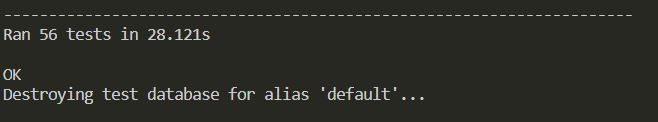
\includegraphics[scale=1]{testresult}
	\caption{A "python manage.py test projects" parancs eredménye.}
	\label{fig:tests}
\end{figure}

Az egység tesztekhez a \textit{test} parancs futtatása során létrejön a memóriában egy ideiglenes adatbázis, amely szerkezetileg megegyezik a valós adatbázissal. 

A \textit{ScrumHelper} minden applikációjában, ahol van szolgáltatás és/vagy nézet réteg (azaz \textit{services.py vagy views.py} fájlok), ott minden funkcióra (függvényre) vonatkozik egy-egy teszteset. Ahol sajátkezűleg szükséges volt megoldani az esetleges hibák lekezelést (tehát nem a keretrendszer működésén múlik), ott egy pozitív (azaz helyes működés) és egy negatív (azaz hiba esetén) teszteset vizsgálja az elvárt működést.

\subsection{Felületi tesztek}

Felületi tesztek automatikus elvégzésére nem biztosít lehetőséget a Django, ezért ezeket a teszteket kézzel, az alábbi forgatókönyvet végig játszva lehet eredményesen letesztelni:

\begin{enumerate}
	\item Bejelentkezés: 
	\begin{itemize}
		\item \textbf{helyes adatok:} A program bejelentkezteti a felhasználót és a főoldalra navigálja.
		\item \textbf{helytelen adatok:} Egy hibaüzenet figyelmezteti a felhasználót a hibás adatokra. Az alkalmazás nem léptet tovább.
		\item \textbf{üres mezők:} Figyelmeztető üzenet az üresen hagyott mezőkre.
		\item \textbf{sikeres bejelentkezés nélkül továbblépés:} Ebben az esetben egy hibaüzenet jelenik meg egy linkkel a bejelentkezési oldalra.
		\item \textbf{Logout menüpont a navigációs sávban:} Kijelentkeztet és visszavezeti a felhasználót a bejelentkező oldalra.
	\end{itemize}
	\item Főoldal:
	\begin{itemize}
		\item \textbf{ScrumHelper szövegre kattintás:} A program bármely oldalról, ha a navigációs sávbeli \textbf{Scrumhelper} szövegre kattintunk, akkor visszajuttat erre a főodlalra.
		\item \textbf{Navigációs sáv menüpontjaira kattintás:} Rendre az elvárt oldalakra navigálnak el.
		\item \textbf{A három menüpont alatti View gombok:} Rendre eljutunk a \textbf{Projects} index oldalra, a saját munkanapló oldalra, valamint a saját profil oldalra.
	\end{itemize}
	\item Projekt index oldal:
	\begin{itemize}
		\item \textbf{Listás megjelenítés:} Valóban egyszerre csak öt (avagy a beállított mennyiségű) projekt jelenik meg a listában.
		\item \textbf{Az oldal léptető gombok:} Megfelelő oldalszámot mutat és valóban tovább ugrik a listán.
		\item \textbf{Működő projekt linkek:} A listában szereplő projektek neve melletti nyíl ikon helyesen a projekt saját oldalára mutat.
	\end{itemize}
	\item Egyes objektumok részletező oldalai:
	\begin{itemize}
		\item \textbf{Felhasználói linkek:} A felhasználóneveket tartalmazó mezők valóban a megfelelő profil oldalára juttatnak el.
		\item \textbf{Dokumentum feltöltés:} Kiválasztó gomb (valamint kiválasztás) és feltöltés működik. Feltöltés után megjelenik a dokumentum a listában.
		\item \textbf{Dokumentum törlés:} A törlés gombra listából eltűnik a dokumentum.
		\item \textbf{Dokumentum linkek:} A dokumentumra kattintva megtekinthetőek a fájlok.
		\item \textbf{Epic, Story, Task, Issue lista:} Az összes feladat típus, ami a projekthez lett létrehozva megjelennek a listában. Az egyes elemre kattitnva eljutunk annak saját oldalára.
		\item \textbf{Almenü (jobb alsó sarok):} Az egeret ráhúzva megjelennek a menüpontok: szerkeztés, issue, story, task és epic létrehozás, munkaidő könyvelés (story, task, issue esetén) valamint megfelelő admin/projekt tulajdonosként törlés.
		\item \textbf{Kommentek létrehozása:} Komment beküldése esetén (ahol erre van lehetőség), a komment megfelelő időponttal, a létrehozó felhasználóhoz kötve (linkkel ellátva), a beírt szöveggel létrejön.
		\item \textbf{Kommentek törlése:} A törlés gombra kattintás határásra a kitörlődik, nem lesz látható.
		\item \textbf{Projekt törlése:} Projekt törlése esetén az összes feladat, amelyet ez alatt hoztak létre törlődik.
	\end{itemize} 
	\item Az egyes létrehozási oldalak (projekt, story, epic, task, issue)
	\begin{itemize}
		\item \textbf{Üres mezők:} Figyelmeztető üzenet a szükséges mezők kitöltésére. Az opcionálisakra nem.
		\item \textbf{Formai ellenőrzés:} Az egyes adatmezők formai ellenőrzése megtörténik. Hiba esetén hibaüzenet.
		\item \textbf{Mentés:} Sikeres kitöltés esetén létrejön az objektum.
	\end{itemize}
	\item Munkanapló
	\begin{itemize}
		\item \textbf{Saját munkanapló oldal:} Dátum kiválasztása előtt az aktuálsi hónaphoz és naphoz jelennek meg a bejegyzések (és csak ehhez). Dátum választás után a megfelelő hónaphoz és naphoz.
		\item \textbf{Hibás input lekérdezésnél:}  Hibaüzenet.
		\item \textbf{Hibás input létrehozásnál:} Dátum formátum ellenrőzés, ennek megfelelő hibaüzenet, avagy nem 1 és 8 közé eső szám megadása esetén is figyelmeztetés.
		\item \textbf{Törlés:} A bejegyzés törlés ikonjára kattintva az eltűnik a felületről (és az adatbázisból is).
		\item \textbf{Scrum munkanapló:} Csak rendszergazda, scrum master és projekt menedzser jogosultságú felhasználó látja mindenki kiszámolt óraszámát a kiválasztott hónapra. A sajátját mindenki látja (a többieknél 0 szerepel).
	\end{itemize}
	\item Kanban
	\begin{itemize}
		\item \textbf{Tartalom:} Az összes olyan story,task,issue, szerepel a táblán, amely nem CLOSED státuszú (és 30 napon belül lett módosítva).
		\item \textbf{Működő linkek:} Az egyes feladatok "kártyájára" kattintva megfelelő linkre jutunk el.
		\item \textbf{Kimutatás:} Megjelenik a kördiagramm és valós arányokat mutat a kanban tábla tekintetében.
	\end{itemize}
	\item Jogosultság kezelés
	\begin{itemize}
		\item \textbf{Csoport lista:} Megjelenik, oldalakra tördelve (ötösével) az összes felhasználói csoport. A léptetés működik.
		\item \textbf{Csoport létrehozás:} Még nem létező csoport létrehozásakor megjelenik az új csoport neve a listában. Létező esetén hibaüzenet.
		\item \textbf{Csoport törlése:} Eltűnik a listából a csoport a törlés gombra kattintás után. Ugyanezen névvel létre lehet hozni újra.
		\item \textbf{Jogosultság hozzáadás és elvétel:} Az egyes csoprotkra kattintva megjelenik a két lista a jogosultsgákokról: az összes éa a csoport aktuális jogai. A plusz gombra kattintva megjelenik a jogosultság az alsó listában. A törlés gombra kattintva eltűnik onnan.
	\end{itemize}
\end{enumerate}